\chapter{Evaluation}\label{chapter:Evaluation}

\section{Graph size}
For evaluating the implementation of the algorithm ... (chan's) in comparison to the brute-force solution, the maximal size of graphs (in $n$) which can be brute-forced in a reasonable time is determined. In general it is favourable to generate as large as possible graphs, for not needing to extrapolate ...
However, the brute forcing time correlates with around $n^8$ (see ...), so with the available resources, it already takes ...s for n=...

For estimating the constant in theorem ..., the a plot of as many grapsh as possible seems to be ideal. So not only for brute-forcing but also for executing algorithm ... oftenly (...), the graph shouldn't be too big, as the (improveable) time complexity of the implementation shows to be at around ... $n...$

As the graphs generated by the algorithms ... have regular? ranks and uniform degrees, it needs to be determined which combination of r and d should be chosen.
For easier evaluation of performance depending on the number of vertices, the rank and degree were chosen to be $r=3$ and $d=3$.
This can't be chosen freely, as For other combinations no r-uniform d-regular graphs exist on .. vertices, as $n d = m r$. This can be verified in the following way: If a "connection" is defined to be the where an edge and a vertex connect, one can count these connections from the vertices' perspective by summing up the degrees of all the vertices (which equals to $n*r$ for uniform/regular graphs). But one can also consider the count of connections from the edges perspective by summing up the ranks of the edges, which equates to $m*r$ for uniform graphs. (todo: source)
As all of the variables in equation... need to be non-negative integers, one can ensure to never violate that constraint for any $n$ by setting $d=r$. 



What time is reasonable is influenced by the following trade-off: either one wants to know the expansion of  

in conclusion 1 minute seems to be a reasinable time for one run of the algorithm.


So the size of the graph is fixed to 20.




In order to not generate very dense graphs but also demonstrate the hypergraph property, the rank of edges is set to 3 and the degree of vertices is set to be ... 




\section{random Generation methods}

As the expansion for not connected graphs is always 0, only algorithms which guarantee connected graphs will be considered.

As it proved difficult to re-generate graphs... only the three algorithms ... , ... and ... will be used. The expansion of the graphs will be evaluated against each other via brute-force and using the approximation alorithm as well.


The edge-weight distribution is always set to be a uniform distribution on $[0.1, 1.1]$
\section{title}

brute forcing not feasibl

todo: analyze size(number vertices) of expansions (depending on k)
analyze expansion quality(number) compared to best expansion possible /average expansion through brute-force for same size
estimate C



TODO: find constants by analyzing quality?
Analyze runtime of code? 

todo: analyze different graph generation algorithms (expansion)

analyze c with different ks, find out which side is more plausible


todo: higher k was not feasible in \cref{eq:small_expansion} due to numerical issues of the implementation, therefore $|S|<\frac{24|V|}{k}$ can't be verified as k<5 here
For estimating $C$, the inequality can be changed to
\begin{equation}
 C\ge \frac {\phi(S)}{ \min\{\sqrt{r \log k}, k \log k  \log \log k \sqrt{\log r} \} \cdot \sqrt{\xi}}
\end{equation}

Knowing an upper bound on C is desirable, as it would lead to small expansions.

\begin{figure}
	\centering
	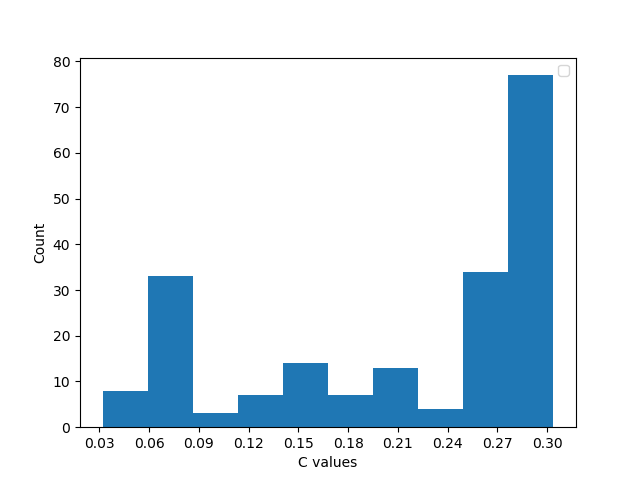
\includegraphics[scale=1]{figures/quality_evaluation_log_C_estimates.png}
	\caption[Plot C]{Plot of C}
\end{figure}